\section{Progettazione concettuale}

\subsection{Diagramma Delle Classi UML}

\begin{figure}[ht]
    \centering
    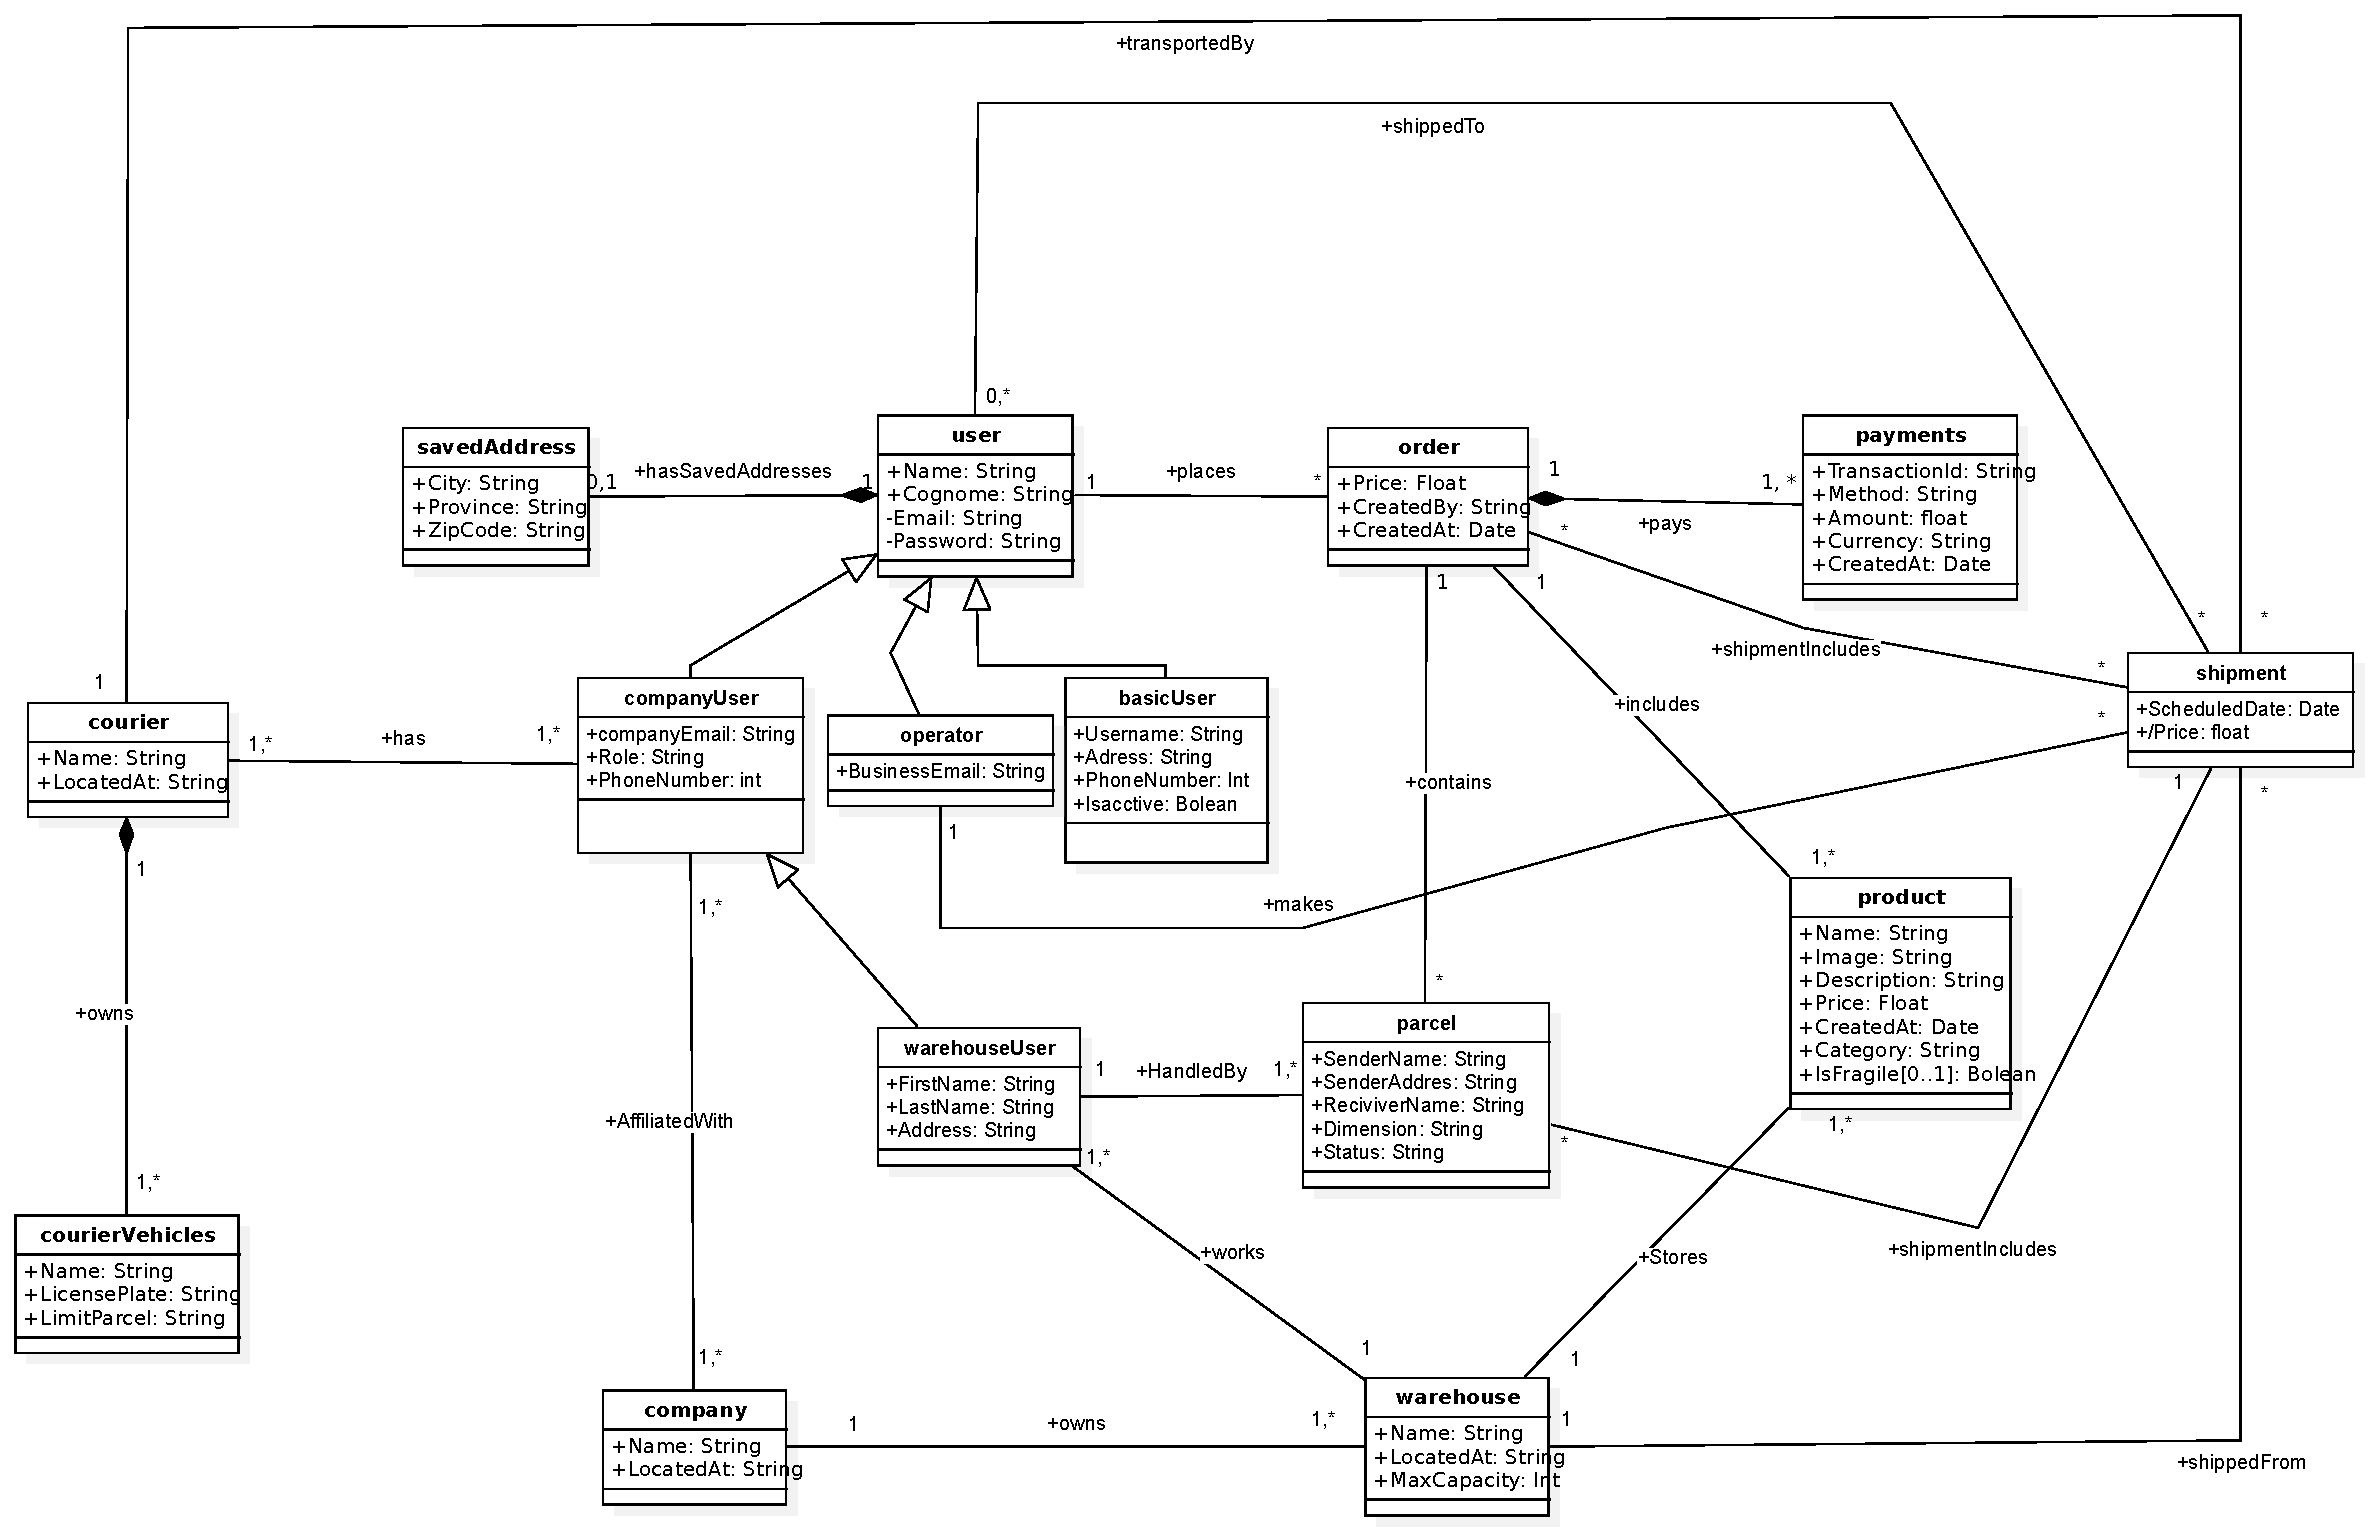
\includegraphics[scale=0.4]{imgs/umlConcettuale.pdf}
    \caption{Diagramma delle classi UML}
\end{figure}

\newpage

\subsection{Leggenda del Diagramma Entità-Relazione}

Nella creazione del diagramma Entità-Relazione, abbiamo impiegato diversi colori per distinguere chiaramente le varie componenti. Per assicurare la chiarezza e facilitare la comprensione del diagramma, di seguito è presentata una leggenda che spiega i simboli usati e i loro colori corrispondenti:
\begin{itemize}[leftmargin=*,label={\textbullet},itemsep=0pt,topsep=0pt,partopsep=0pt]
    \item \textbf{Entità}:
          \begin{itemize}[leftmargin=*,label={\textbullet},itemsep=0pt,topsep=0pt,partopsep=0pt]
            \item \textbf{Rettangolo Azzurro}:  Rappresenta un'entità. Il nome dell'entità è posizionato all'interno del rettangolo;
            \item \textbf{Rettangolo Grigio con doppia linea}: Indica un'entità debole.
          \end{itemize}
    \item \textbf{Attributo}:
          \begin{itemize}[leftmargin=*,label={\textbullet},itemsep=0pt,topsep=0pt,partopsep=0pt]
            \item \textbf{Ovale Giallo}: Rappresenta un attributo. Il nome dell'attributo è posizionato all'interno dell'ovale;
            \item \textbf{Ovale tratteggiato}: Indica un attributo derivato;
            \item \textbf{Nome sottolineato}: Indica un attributo chiave.
          \end{itemize}
    \item \textbf{Relazione}:
          \begin{itemize}[leftmargin=*,label={\textbullet},itemsep=0pt,topsep=0pt,partopsep=0pt]
            \item \textbf{Rombo Verde}: Rappresenta una relazione. Il nome della relazione è posizionato all'interno del rombo;
            \item \textbf{Rombo con Doppia Linea}: Indica una relazione di tipo debole.
          \end{itemize}
    \item \textbf{Specializzazioni}:
          \begin{itemize}[leftmargin=*,label={\textbullet},itemsep=0pt,topsep=0pt,partopsep=0pt]
            \item \textbf{Cerchio e Linea Rosa}: Rappresentano una specializzazione.
                  \begin{itemize}[leftmargin=*,label={\textbullet},itemsep=0pt,topsep=0pt,partopsep=0pt]
                    \item \textbf{Lettera "U" (Magnete)}: Indica la direzione della sottoclasse nella specializzazione;
                    \item \textbf{Lettera "d"}: Specifica una specializzazione disgiunta;
                    \item \textbf{Lettera "o"}: Specifica una specializzazione overlapping;
                    \item \textbf{Singola Linea}: Rappresenta la parzialità della specializzazione;
                    \item \textbf{Doppia Linea}: Rappresenta la totalità della specializzazione.
                  \end{itemize}
          \end{itemize}
\end{itemize}

\newpage

\subsection{Diagramma Entità-Relazione}

\begin{figure}[ht]
    \centering
    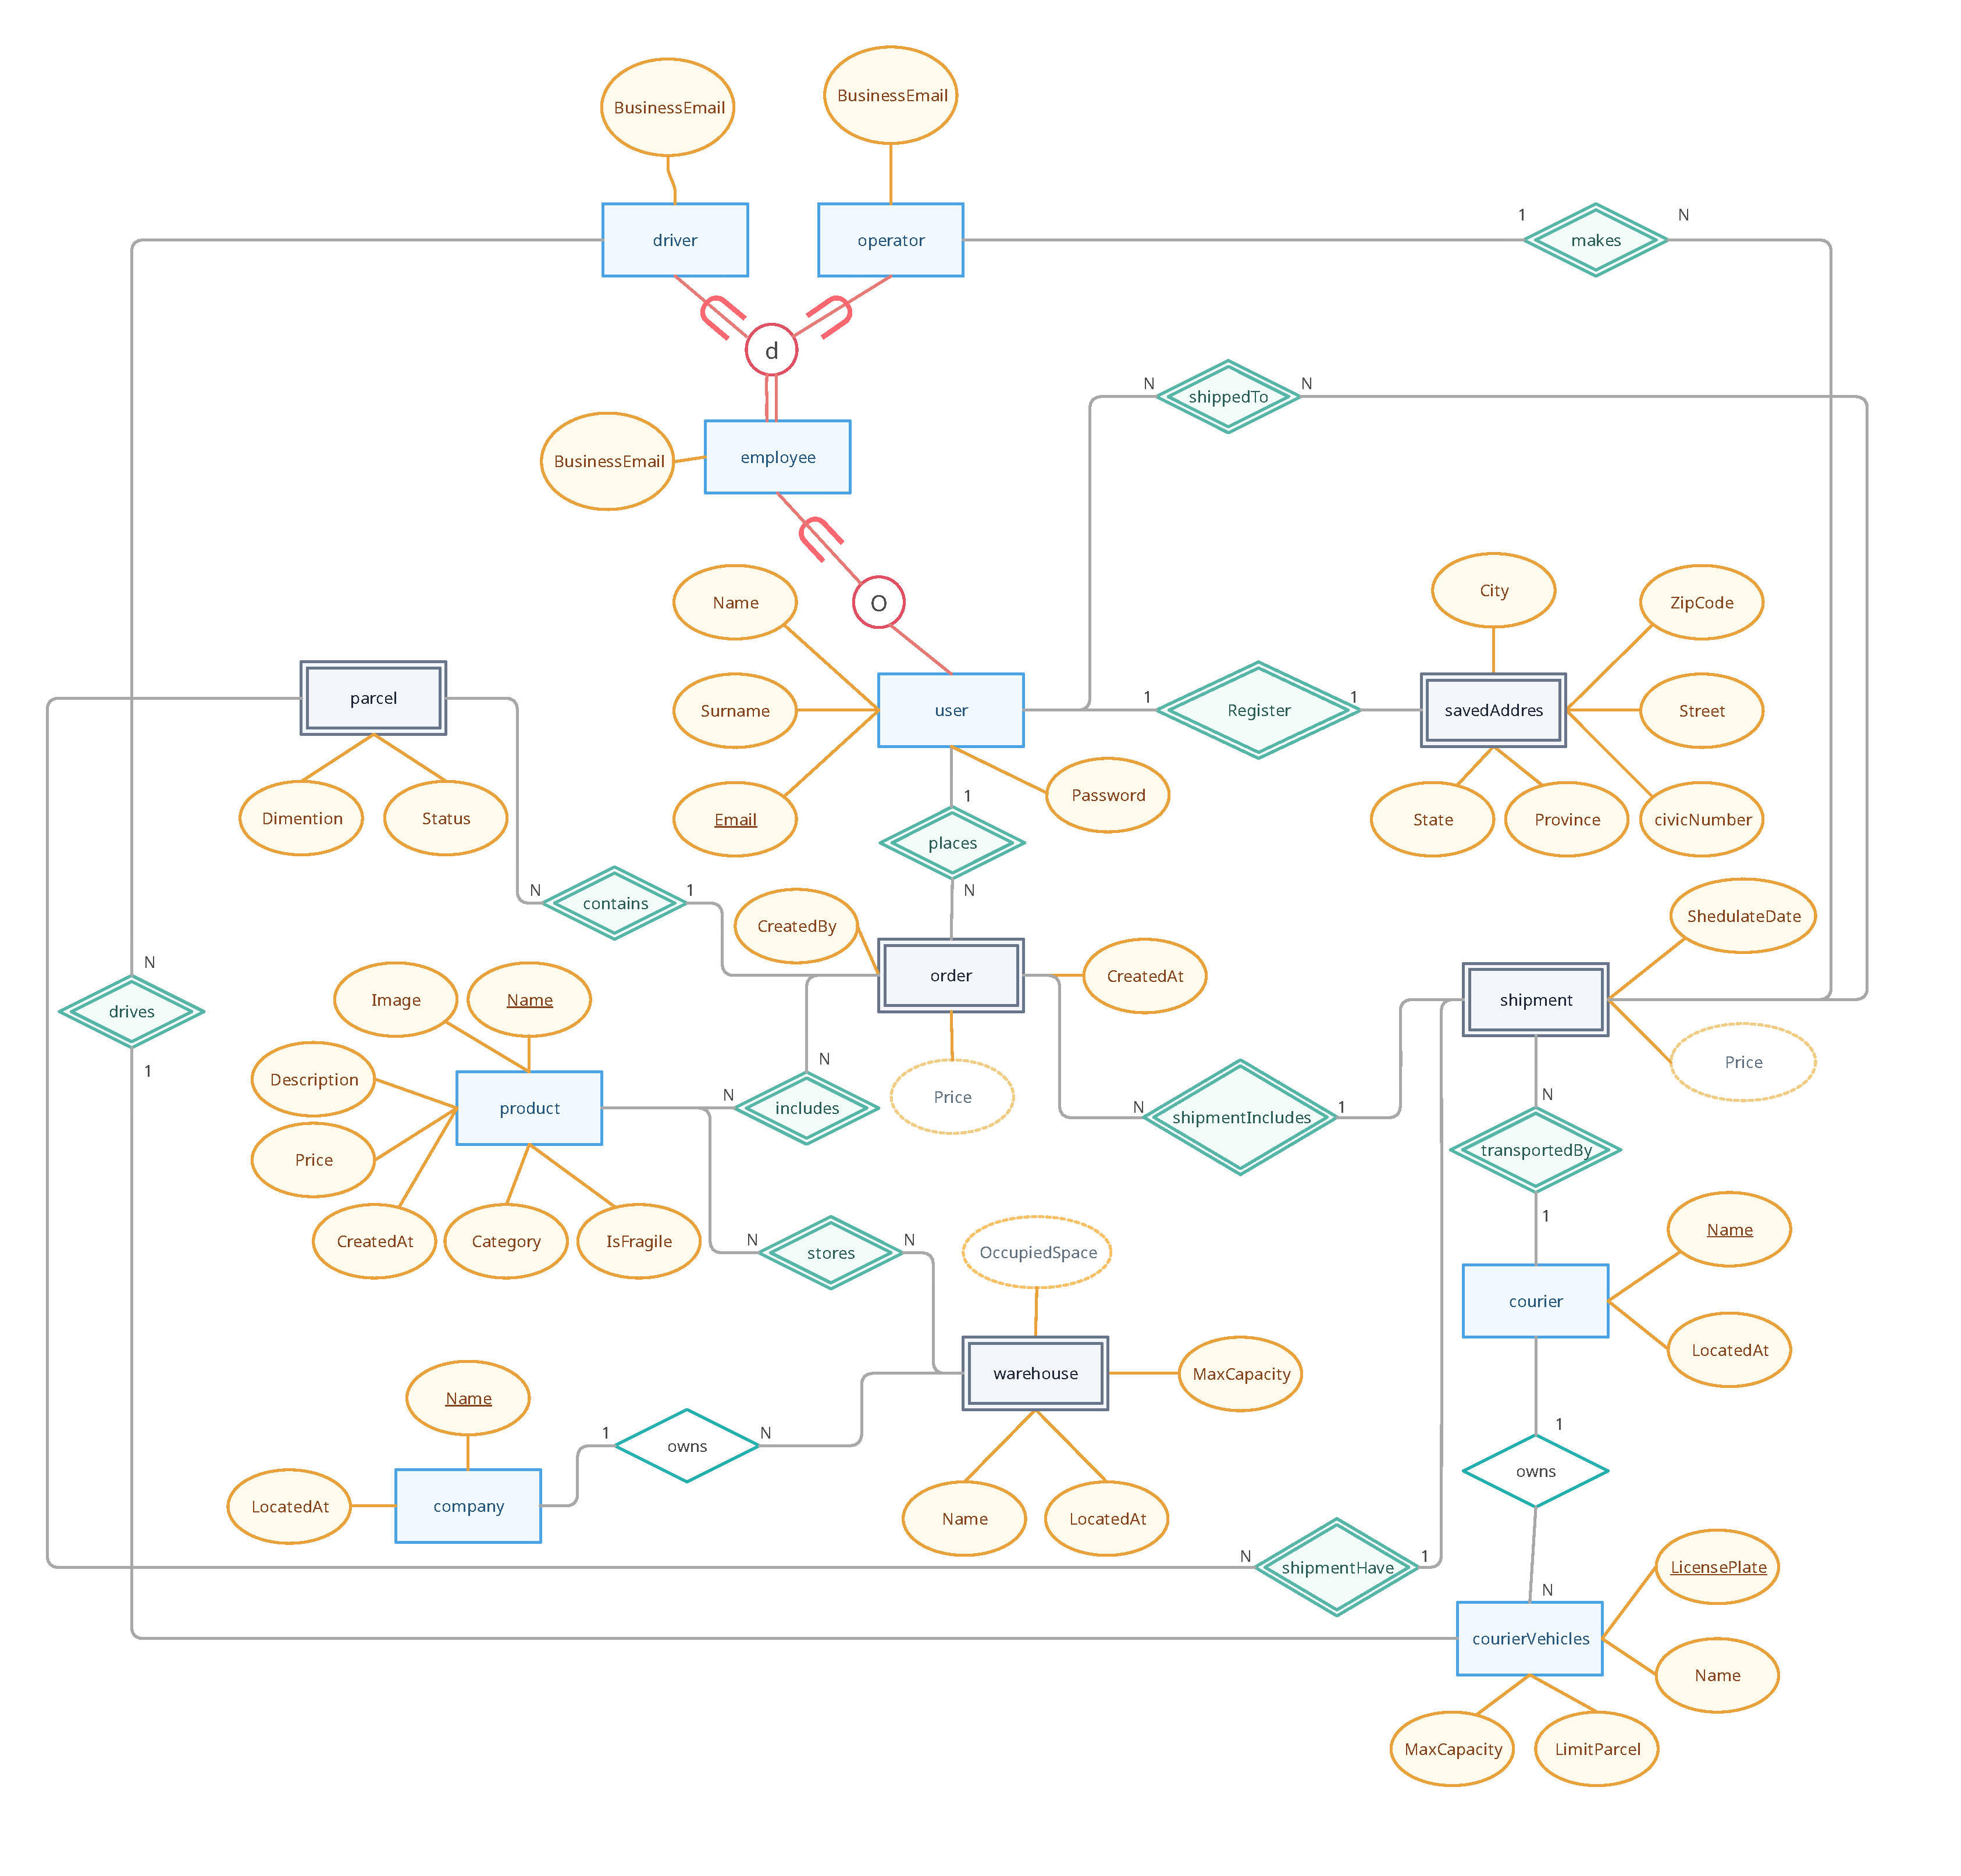
\includegraphics[scale=0.30]{imgs/er.pdf}
    \caption{Diagramma Entità-Relazione}
\end{figure}

\newpage

\section{Ristrutturazione}

\subsection{Considerazioni}

\subsubsection{Attributi Multivalore e Composti}

Durante la fase di progettazione concettuale del database, è stata presa una decisione riguardo agli attributi multivalore e composti. Abbiamo scelto di evitare l'uso di attributi multivalore o composti. Questa decisione è stata guidata dalla necessità di mantenere una struttura di database chiara e di facile gestione.

\subsubsection{Specializzazioni}

Le varie \textbf{specializzazioni} e le varie \textbf{generalizzazioni} sono state modellate nei seguenti modi:

\begin{itemize}[leftmargin=*,label={\textbullet},itemsep=0pt,topsep=0pt,partopsep=0pt]
    \item \textbf{Employee}:
          \begin{itemize}[leftmargin=*,label={\textbullet},itemsep=0pt,topsep=0pt,partopsep=0pt]
            \item \textbf{Tipo di Specializzazione}: Totale e disgiunta;
            \item \textbf{Implementazione}: Abbiamo scelto di accorpare la classe generale \textbf{Employee} in classi specializzate.
          \end{itemize}
    \item \textbf{Account}:
          \begin{itemize}[leftmargin=*,label={\textbullet},itemsep=0pt,topsep=0pt,partopsep=0pt]
            \item \textbf{Tipo di Specializzazione}: Parziale e Totale;
            \item \textbf{Implementazione}: Per la specializzazione di \textbf{Account}, abbiamo deciso di trasformarla in un'associazione. Questo approccio ci ha permesso di limitare i vincoli d'integrità e di gestire in modo più efficace i campi che possono assumere valori null.
          \end{itemize}
\end{itemize}

\subsubsection{Attributi Derivati}

Nel contesto della progettazione concettuale del database, abbiamo implementato tre attributi derivati, gestendoli nel seguente modo:

\begin{itemize}[leftmargin=*,label={\textbullet},itemsep=0pt,topsep=0pt,partopsep=0pt]
    \item \textbf{Attributo Price}:
          \begin{itemize}[leftmargin=*,label={\textbullet},itemsep=0pt,topsep=0pt,partopsep=0pt]
            \item \textbf{Gestione}: Nonostante \textbf{Price} sia un attributo derivato (tipicamente calcolato a partire da altri dati), abbiamo deciso di conservarlo direttamente nel nostro sistema.
            \item \textbf{Motivazione}: Questa scelta è stata fatta per ottimizzare le prestazioni del sistema, evitando il calcolo ripetuto dei prezzi ogni volta che vengono richiesti. Conservando il prezzo calcolato, riduciamo il carico sul sistema e miglioriamo l'efficienza delle query.
          \end{itemize}
    \item \textbf{Attributo OccupiedSpace}:
          \begin{itemize}[leftmargin=*,label={\textbullet},itemsep=0pt,topsep=0pt,partopsep=0pt]
            \item \textbf{Gestione}: Abbiamo scelto di conservare anche l'attributo \textbf{OccupiedSpace} all'interno del nostro sistema.
            \item \textbf{Motivazione}: Questa decisione è stata presa considerando l'importanza di questo attributo, che può essere frequentemente richiesto dal sistema per la gestione degli spazi nei magazzini. Conservandolo, siamo in grado di fornire rapidamente le informazioni richieste senza la necessità di calcoli aggiuntivi.
          \end{itemize}
\end{itemize}

\newpage

\subsubsection{Analisi delle Ridondanze}

Nel processo di ottimizzazione del database, abbiamo eseguito un'analisi dettagliata per identificare e risolvere eventuali ridondanze.

\begin{itemize}[leftmargin=*,label={\textbullet},itemsep=0pt,topsep=0pt,partopsep=0pt]
  \item \textbf{Ridondanza negli attributi delle associazioni}:
        \begin{itemize}[leftmargin=*,label={\textbullet},itemsep=0pt,topsep=0pt,partopsep=0pt]
          \item \textbf{Situazione Identificata}: Dopo la ristrutturazione delle specializzazioni, abbiamo riscontrato la presenza di ridondanza negli attributi. In particolare, l'attributo \textbf{BusinessEmail} era presente sia nell'associazione \textbf{Driver} che in \textbf{Operators}, pur essendo associato a due entità diverse.
          \item \textbf{Soluzione Implementata}: Per risolvere questa ridondanza, abbiamo introdotto attributi identificativi specifici per ciascuna associazione. Nell'associazione \textbf{Driver}, è stato aggiunto l'attributo \textbf{driverId} per identificare univocamente ogni driver. Analogamente, nell'associazione \textbf{Operators}, è stato introdotto \textbf{operatorId} per l'identificazione univoca degli operatori.
        \end{itemize}
  \item \textbf{Ambiguità nei nomi delle relazioni}:
        \begin{itemize}[leftmargin=*,label={\textbullet},itemsep=0pt,topsep=0pt,partopsep=0pt]
          \item \textbf{Situazione Identificata}: Abbiamo notato una sovrapposizione nei nomi delle relazioni tra \textbf{Orders} e \textbf{Shipment} e tra \textbf{Parcel} e \textbf{Shipment}. Nonostante avessero lo stesso nome, queste relazioni indicavano relazioni sostanzialmente diverse.
          \item \textbf{Soluzione Implementata}: Per eliminare questa ambiguità, abbiamo deciso di rinominare la relazione tra \textbf{Orders} e \textbf{Shipment} in \textbf{orderShipment}. Questo aiuta a distinguere chiaramente questa relazione da quella tra \textbf{Parcel} e \textbf{Shipment}.
        \end{itemize}
\end{itemize}

\subsubsection{Identificazione delle Chiavi Primarie}

Abbiamo effettuato delle scelte riguardo all'uso di chiavi primarie, in particolare l'introduzione di chiavi surrogate in alcune associazioni chiave.

\begin{itemize}[leftmargin=*,label={\textbullet},itemsep=0pt,topsep=0pt,partopsep=0pt]
  \item \textbf{Associazione Orders}:
        \begin{itemize}[leftmargin=*,label={\textbullet},itemsep=0pt,topsep=0pt,partopsep=0pt]
          \item \textbf{Decisione}: Introduzione di una chiave surrogata per identificare univocamente ogni ordine chiamata \textbf{OrderId}.
          \item \textbf{Motivazione}: L'uso di una chiave surrogata in questa associazione assicura che ogni ordine registrato nel sistema sia univoco. Questo non solo semplifica la gestione e il tracciamento degli ordini attuali, ma apre anche la strada per un potenziale supporto di funzionalità avanzate, come la gestione di ordini multipli o complessi in futuro.
        \end{itemize}
  \item \textbf{Associazioni Driver e Operators}:
        \begin{itemize}[leftmargin=*,label={\textbullet},itemsep=0pt,topsep=0pt,partopsep=0pt]
          \item \textbf{Decisione}: Aggiunta di chiavi surrogate in entrambe le associazioni, come menzionato nell'analisi delle ridondanze.
          \item \textbf{Motivazione}: Questa scelta è stata guidata dall'analisi della ridondanza, garantendo un'identificazione chiara e distinta di ogni driver e ogni operatore.
        \end{itemize}
  \item \textbf{Associazione Company}:
        \begin{itemize}[leftmargin=*,label={\textbullet},itemsep=0pt,topsep=0pt,partopsep=0pt]
          \item \textbf{Decisione}: Introduzione di una chiave surrogata nell'associazione \textbf{Company}, chiamata \textbf{CompanyId}.
          \item \textbf{Motivazione}: Abbiamo identificato la necessità di un identificatore unico più affidabile del solo nome aziendale, avendo riscontrato casi di aziende con lo stesso nome. La chiave surrogata assicura una distinzione precisa tra le aziende, anche in presenza di nomi omonimi.
        \end{itemize}
\end{itemize}

\newpage

\subsubsection{Diagramma Delle Classi UML Ristrutturato}

\begin{figure}[ht]
  \centering
  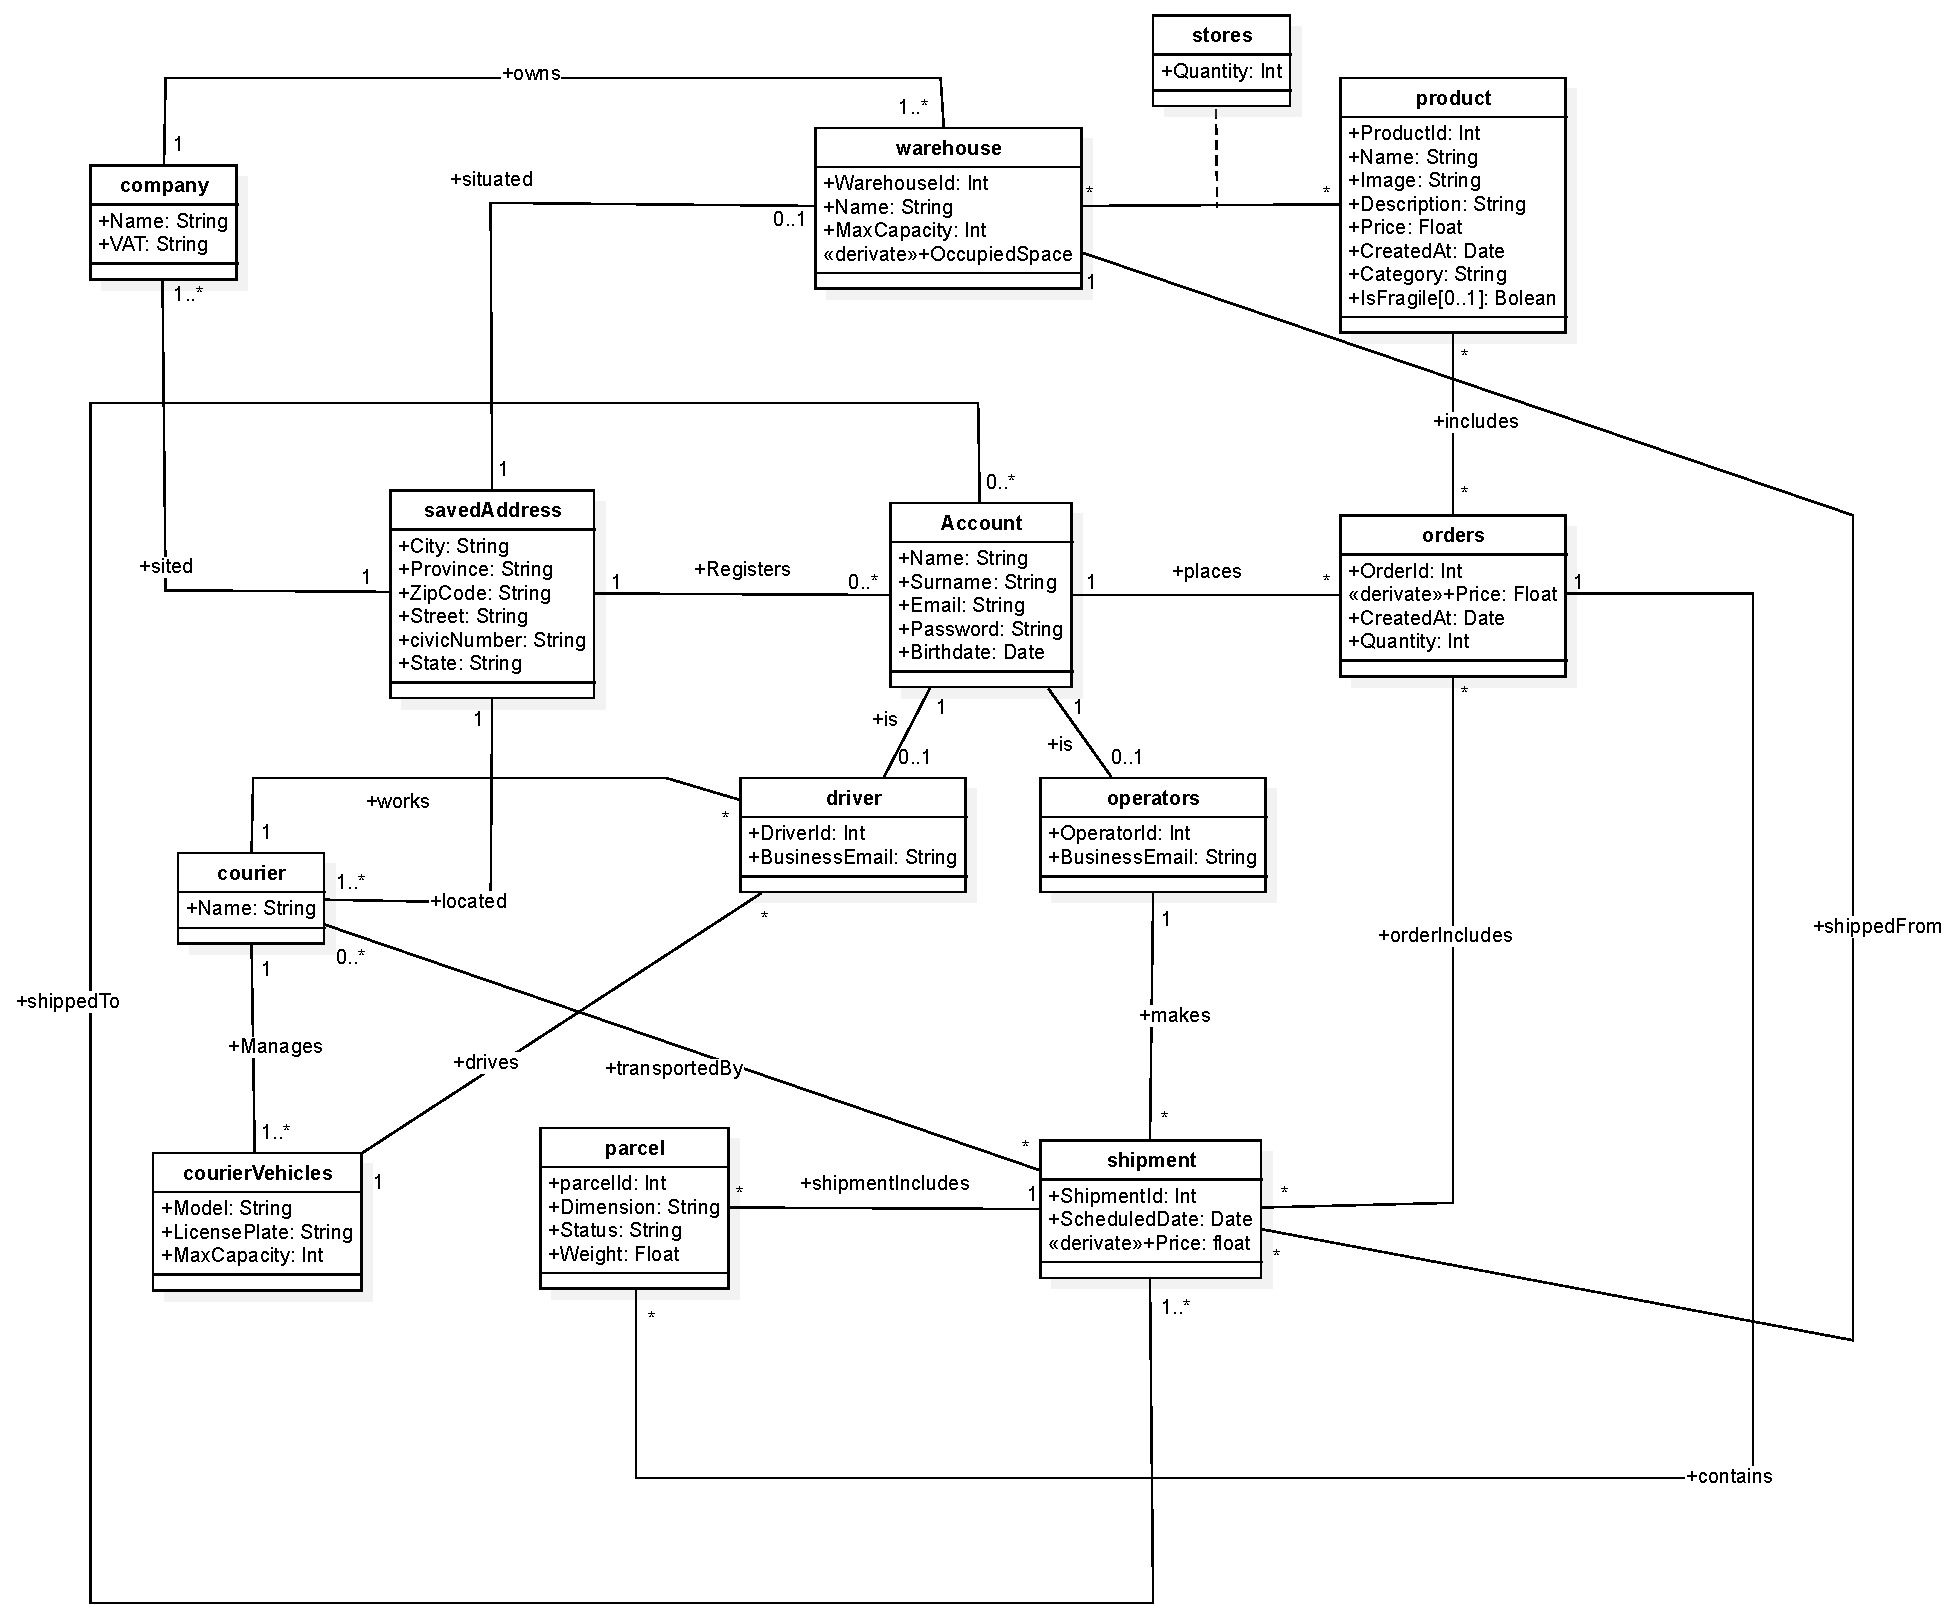
\includegraphics[scale=0.55]{imgs/umlRistrutturato.pdf}
  \caption{Diagramma delle classi UML Ristrutturato}
\end{figure}

\newpage

\subsection{Dizionari}

\subsubsection{Dizionario delle Classi}

\rowcolors{2}{white}{lightgray}
\begin{tabularx}{\textwidth}{YYY}
  \toprule
  \textbf{Classe} & \textbf{Descrizione} & \textbf{Attributi} \\
  \midrule
  Account & Utente generico che utilizza il sistema &
  \begin{minipage}[c]{\linewidth}%
    \vspace{0.45cm}
    \footnotesize
    \textbf{Name}: Nome dell'utente; \newline
    \textbf{Surname}: Cognome dell'utente; \newline
    \textbf{Email}: Indirizzo email (chiave primaria); \newline
    \textbf{Password}: Password dell'utente. \newline
    \textbf{Birthdate}: Data di nascita dell'utente; \newline
  \end{minipage} \\
  SavedAddress & Conserva gli indirizzi salvati dagli utenti &
  \begin{minipage}[c]{\linewidth}%
    \vspace{0.45cm}
    \footnotesize
    \textbf{City}: Città in cui risiede l'utente; \newline
    \textbf{Province}: Provincia in cui risiede l'utente; \newline
    \textbf{ZipCode}: Codice postale della città in cui risiede l'utente; \newline
    \textbf{Street}: Via in cui risiede l'utente; \newline
    \textbf{CivicNumber}: Numero civico della via in cui risiede l'utente; \newline
    \textbf{State}: Stato in cui risiede l'utente; \newline
  \end{minipage} \\
  Orders & Rappresenta un ordine effettuato da un utente &
  \begin{minipage}[c]{\linewidth}%
    \vspace{0.45cm}
    \footnotesize
    \textbf{OrderId}: Identificatore univoco (chiave primaria); \newline
    \textbf{CreatedBy}: Utente che ha creato l'ordine; \newline
    \textbf{Price}: Prezzo totale. \newline
    \textbf{Quantity}: Quantità di prodotti ordinati. \newline
  \end{minipage} \\
  Operators & Account di un impiegato che gestisce gli ordini &
  \begin{minipage}[c]{\linewidth}%
    \vspace{0.45cm}
    \footnotesize
    \textbf{operatorId}:  Identificatore univoco (chiave primaria); \newline
    \textbf{BusinessEmail}: Email aziendale. \newline
  \end{minipage} \\
  Driver & Account di un autista che consegna gli ordini &
  \begin{minipage}[c]{\linewidth}%
    \vspace{0.45cm}
    \footnotesize
    \textbf{driverId}: Identificatore univoco (chiave primaria); \newline
    \textbf{BusinessEmail}: Email aziendale. \newline
  \end{minipage} \\
  Company & Rappresenta un'azienda che vende prodotti &
  \begin{minipage}[c]{\linewidth}%
    \vspace{0.45cm}
    \footnotesize
    \textbf{Name}: Nome dell'azienda; \newline
    \textbf{VAT}: Partita IVA dell'azienda (chiave primaria). \newline
  \end{minipage} \\
  Warehouse & Rappresenta un magazzino di un'azienda &
  \begin{minipage}[c]{\linewidth}%
    \vspace{0.45cm}
    \footnotesize
    \textbf{WarehouseId}:  Identificatore univoco (chiave primaria); \newline
    \textbf{Name}: Nome del magazzino; \newline
    \textbf{MaxCapacity}: Capacità massima del magazzino; \newline
    \textbf{OccupiedSpace}: Spazio occupato attualmente nel magazzino. \newline
  \end{minipage} \\
  Shipment & Rappresenta una spedizione &
  \begin{minipage}[c]{\linewidth}%
    \vspace{0.5cm}
    \footnotesize
    \textbf{ShipmentId}: Identificatore univoco (chiave primaria); \newline
    \textbf{ScheduledDate}: Data prevista consegna; \newline
    \textbf{Price}: Prezzo della spedizione. \newline
  \end{minipage} \\
  \bottomrule
\end{tabularx}

\rowcolors{2}{white}{lightgray}
\begin{tabularx}{\textwidth}{YYY}
  \toprule
  \textbf{Classe} & \textbf{Descrizione} & \textbf{Attributi} \\
  \midrule
  Product & Rappresenta un singolo prodotto venduto da un'azienda &
  \begin{minipage}[c]{\linewidth}%
    \vspace{0.5cm}
    \footnotesize
    \textbf{productId}: Identificatore univoco (chiave primaria); \newline
    \textbf{Name}: Nome del prodotto; \newline
    \textbf{Image}: Eventuale Immagine del prodotto; \newline
    \textbf{Description}: Descrizione del prodotto; \newline
    \textbf{Price}: Prezzo del prodotto; \newline
    \textbf{CreatedAt}: Data di creazione del prodotto; \newline
    \textbf{Category}: Categoria del prodotto; \newline
    \textbf{IsFragile}: Indica se il prodotto è fragile. \newline
  \end{minipage} \\
  Parcel & Rappresenta il pacco da spedire &
  \begin{minipage}[c]{\linewidth}%
    \vspace{0.5cm}
    \footnotesize
    \textbf{ParcelId}: Identificatore univoco (chiave primaria); \newline
    \textbf{Dimention}: Dimensione del pacco; \newline
    \textbf{Weight}: Peso del pacco; \newline
    \textbf{Status}: Stato del pacco. \newline
  \end{minipage} \\
  Courier & Rappresenta un corriere &
  \begin{minipage}[c]{\linewidth}%
    \vspace{0.35cm}
    \footnotesize
    \textbf{Name}: Nome del corriere (chiave primaria). \newline
  \end{minipage} \\
  CourierVehicle & \vspace{-0.5cm}Rappresenta un veicolo utilizzato da un corriere &
  \begin{minipage}[c]{\linewidth}%
    \vspace{0.5cm}
    \footnotesize
    \textbf{Model}: Modello del veicolo; \newline
    \textbf{LicensePlate}: Targa del veicolo (chiave primaria); \newline
    \textbf{MaxCapacity}: Capacità massima del veicolo. \newline
  \end{minipage} \\
  \bottomrule
\end{tabularx}

\subsubsection{Dizionario delle Associazioni}

\rowcolors{2}{white}{lightgray}

\begin{tabularx}{\textwidth}{YYY}
  \toprule
  \textbf{Associazione} & \textbf{Descrizione} & \textbf{Classi Coinvolte} \\
  \midrule
  Places &
  \begin{minipage}[c]{\linewidth}
    \vspace{0.5cm}
    Rappresenta la relazione tra un \textbf{Account} e un \textbf{Orders}. \newline
  \end{minipage} &
  \begin{minipage}[c]{\linewidth}
    \vspace{0.5cm}
    \textbf{Account} [\(1\)] (places): L'account che effettua un ordine; \newline
    \textbf{Orders} [\(*\)] (placed by): Gli ordini effettuati da un account. \newline
  \end{minipage} \\

  Registers &
  \begin{minipage}[c]{\linewidth}
    \vspace{0.5cm}
    Rappresenta la relazione tra un \textbf{Account} e un \textbf{SavedAddress}. \newline
  \end{minipage} &
  \begin{minipage}[c]{\linewidth}
    \vspace{0.5cm}
    \textbf{Account} [\(0..1\)] (Registers):  L'account che ha salvato l'indirizzo; \newline
    \textbf{SavedAddress} [\(1\)] (isRegistersBy): Gli indirizzi salvati da un account. \newline
  \end{minipage} \\

  Is &
  \begin{minipage}[c]{\linewidth}
    \vspace{0.5cm}
    Rappresenta la relazione tra un \textbf{Account} e un \textbf{Operators}. \newline
  \end{minipage} &
  \begin{minipage}[c]{\linewidth}
    \vspace{0.5cm}
    \textbf{Account} [\(1\)] (Is): L'account identificato come utente; \newline
    \textbf{Operators} [\(0..1\)] (has): Gli operatori associati a un account. \newline
  \end{minipage} \\

  Is &
  \begin{minipage}[c]{\linewidth}
    \vspace{0.5cm}
    Rappresenta la relazione tra un \textbf{Account} e un \textbf{Driver}. \newline
  \end{minipage} &
  \begin{minipage}[c]{\linewidth}
    \vspace{0.5cm}
    \textbf{Account} [\(1\)] (Is):  L'account identificato come utente; \newline
    \textbf{Driver} [\(0..1\)] (has): I driver associati a un account. \newline
  \end{minipage} \\
  \bottomrule
\end{tabularx}

\newpage

\rowcolors{2}{white}{lightgray}
\begin{tabularx}{\textwidth}{YYY}
  \toprule
  \textbf{Associazione} & \textbf{Descrizione} & \textbf{Classi Coinvolte} \\
  \midrule
  Owns &
  \begin{minipage}[c]{\linewidth}
    \vspace{0.5cm}
    Rappresenta la relazione tra un \textbf{Company} e un \textbf{Warehouse}. \newline
  \end{minipage} &
  \begin{minipage}[c]{\linewidth}
    \vspace{0.5cm}
    \textbf{Company} [\(1\)] (owns): La compagnia che possiede il magazzino; \newline
    \textbf{Warehouse} [\(1..*\)] (owned by):  I magazzini posseduti da una data compagnia. \newline
  \end{minipage} \\

  ShippedFrom &
  \begin{minipage}[c]{\linewidth}
    \vspace{0.5cm}
    Rappresenta la relazione tra un \textbf{Warehouse} e un \textbf{Shipment}. \newline
  \end{minipage} &
  \begin{minipage}[c]{\linewidth}
    \vspace{0.5cm}
    \textbf{Warehouse} [\(1\)]  (shippedFrom):  Il magazzino da cui parte la spedizione; \newline
    \textbf{Shipment} [\(*\)] (comes from): Le spedizioni partite da un dato magazzino. \newline
  \end{minipage} \\

  TransportedBy &
  \begin{minipage}[c]{\linewidth}
    \vspace{0.5cm}
    Rappresenta la relazione tra un \textbf{Shipment} e un \textbf{Courier}. \newline
  \end{minipage} &
  \begin{minipage}[c]{\linewidth}
    \vspace{0.5cm}
    \textbf{Shipment} [\(*\)]  (transportedBy): Le spedizioni effettuate; \newline
    \textbf{Courier} [\(0..*\)] (transports): I corrieri che trasportano le spedizioni. \newline
  \end{minipage} \\

  ShippedTo &
  \begin{minipage}[c]{\linewidth}
    \vspace{0.5cm}
    Rappresenta la relazione tra un \textbf{Shipment} e un \textbf{Account}. \newline
  \end{minipage} &
  \begin{minipage}[c]{\linewidth}
    \vspace{0.5cm}
    \textbf{Shipment} [\(1..*\)]  (shippedTo): Le spedizioni effettuate; \newline
    \textbf{Account} [\(0..*\)] (receives): Gli utenti destinatari delle spedizioni. \newline
  \end{minipage} \\

  OrderIncludes &
  \begin{minipage}[c]{\linewidth}
    \vspace{0.5cm}
    Rappresenta la relazione tra un \textbf{Orders} e un \textbf{Shipment}. \newline
  \end{minipage} &
  \begin{minipage}[c]{\linewidth}
    \vspace{0.5cm}
    \textbf{Orders} [\(*\)]  (ordersIncludedIn): Ordini inclusi nella spedizione; \newline
    \textbf{Shipment} [\(*\)] (shipmentsContaining): Spedizioni che includono gli ordini. \newline
  \end{minipage} \\

  ShipmentIncludes &
  \begin{minipage}[c]{\linewidth}
    \vspace{0.5cm}
    Rappresenta la relazione tra un \textbf{Shipment} e un \textbf{Parcel}. \newline
  \end{minipage} &
  \begin{minipage}[c]{\linewidth}
    \vspace{0.5cm}
    \textbf{Shipment} [\(1\)]  (shipmentsIncluding): Spedizioni che includono pacchi; \newline
    \textbf{Parcel} [\(*\)] (parcelsIncludedIn): Pacchi inclusi nelle spedizioni. \newline
  \end{minipage} \\

  Stores &
  \begin{minipage}[c]{\linewidth}
    \vspace{0.5cm}
    Rappresenta la relazione tra un \textbf{Warehouse} e un \textbf{Product}. \newline
  \end{minipage} &
  \begin{minipage}[c]{\linewidth}
    \vspace{0.5cm}
    \textbf{Warehouse} [\(*\)]  (stores): Magazzini che immagazzinano prodotti; \newline
    \textbf{Product} [\(*\)] (is stored): Prodotti conservati nel magazzino. \newline
  \end{minipage} \\

  Includes &
  \begin{minipage}[c]{\linewidth}
    \vspace{0.5cm}
    Rappresenta la relazione tra un \textbf{Orders} e un \textbf{Product}. \newline
  \end{minipage} &
  \begin{minipage}[c]{\linewidth}
    \vspace{0.5cm}
    \textbf{Orders} [\(1\)]  (is included): Ordini che includono prodotti; \newline
    \textbf{Product} [\(1..*\)] (includes): Prodotti inclusi negli ordini. \newline
  \end{minipage} \\
  \bottomrule
\end{tabularx}

\newpage

\begin{tabularx}{\textwidth}{YYY}
  \toprule
  \textbf{Associazione} & \textbf{Descrizione} & \textbf{Classi Coinvolte} \\
  \midrule
  Contains &
  \begin{minipage}[c]{\linewidth}
    \vspace{0.5cm}
    Rappresenta la relazione tra un \textbf{Orders} e un \textbf{Parcel}. \newline
  \end{minipage} &
  \begin{minipage}[c]{\linewidth}
    \vspace{0.5cm}
    \textbf{Orders} [\(1\)]  (contains): Ordini che contengono pacchi; \newline
    \textbf{Parcel} [\(*\)] (is contained): Pacchi inclusi negli ordini. \newline
  \end{minipage} \\

  Drives &
  \begin{minipage}[c]{\linewidth}
    \vspace{0.5cm}
    Rappresenta la relazione tra un \textbf{Driver} e un \textbf{CourierVehicle}. \newline
  \end{minipage} &
  \begin{minipage}[c]{\linewidth}
    \vspace{0.5cm}
    \textbf{Driver} [\(*\)]  (drives):  Conducenti che guidano veicoli; \newline
    \textbf{CourierVehicle} [\(1\)] (is drived): Veicoli guidati dai conducenti. \newline
  \end{minipage} \\

  Manages &
  \begin{minipage}[c]{\linewidth}
    \vspace{0.5cm}
    Rappresenta la relazione tra un \textbf{CourierVehicle} e un \textbf{Courier}. \newline
  \end{minipage} &
  \begin{minipage}[c]{\linewidth}
    \vspace{0.5cm}
    \textbf{CourierVehicle} [\(1..*\)]  (isManagesBy): Veicoli utilizzati dai corrieri; \newline
    \textbf{Courier} [\(1\)] (manages): Corrieri che hanno i veicoli. \newline
  \end{minipage} \\

  Makes &
  \begin{minipage}[c]{\linewidth}
    \vspace{0.5cm}
    Rappresenta la relazione tra un \textbf{Operators} e un \textbf{Shipment}. \newline
  \end{minipage} &
  \begin{minipage}[c]{\linewidth}
    \vspace{0.5cm}
    \textbf{Operators} [\(1..*\)]  (makes): Operatori che organizzano spedizioni; \newline
    \textbf{Shipment} [\(1\)] (is made): Spedizioni organizzate dagli operatori. \newline
  \end{minipage} \\

  Sited &
  \begin{minipage}[c]{\linewidth}
    \vspace{0.5cm}
    Rappresenta la relazione tra \textbf{Company} e \textbf{SavedAddress}. \newline
  \end{minipage} &
  \begin{minipage}[c]{\linewidth}
    \vspace{0.5cm}
    \textbf{Company} [\(1\)]  (sited): Aziende che hanno sedi; \newline
    \textbf{SavedAddress} [\(1..*\)] (is sited in): Sedi delle aziende. \newline
  \end{minipage} \\

  Located &
  \begin{minipage}[c]{\linewidth}
    \vspace{0.5cm}
    Rappresenta la relazione tra \textbf{Courier} e \textbf{SavedAddress}. \newline
  \end{minipage} &
  \begin{minipage}[c]{\linewidth}
    \vspace{0.5cm}
    \textbf{Courier} [\(1\)]  (located): Corrieri che hanno sedi; \newline
    \textbf{SavedAddress} [\(1..*\)] (is located in): Sedi dei corrieri. \newline
  \end{minipage} \\

  Works &
  \begin{minipage}[c]{\linewidth}
    \vspace{0.5cm}
    Rappresenta la relazione tra \textbf{Driver} e \textbf{Courier}. \newline
  \end{minipage} &
  \begin{minipage}[c]{\linewidth}
    \vspace{0.5cm}
    \textbf{Driver} [\(1\)]  (works): Conducenti che lavorano per corrieri; \newline
    \textbf{Courier} [\(1\)] (employs): Corrieri che impiegano conducenti. \newline
  \end{minipage} \\
  \bottomrule
\end{tabularx}

\subsubsection{Dizionario dei Vincoli}

\begin{tabularx}{\textwidth}{YYYY}
  \toprule
  \textbf{Vincolo} & \textbf{Classi Coinvolte} & \textbf{Tipo} & \textbf{Descrizione} \\
  \midrule
  alfanumName & Account & Dominio &
  \begin{minipage}[c]{\linewidth}
    \vspace{0.5cm}
    Il nome dell'utente deve contenere solo caratteri alfanumerici (lettere e numeri). \newline
  \end{minipage} \\
  alfanumSurname & Account & Dominio &
  \begin{minipage}[c]{\linewidth}
    \vspace{0.5cm}
    Il cognome dell'utente deve includere solamente caratteri alfanumerici. \newline
  \end{minipage} \\
  alfnumEmail & Account & Dominio &
  \begin{minipage}[c]{\linewidth}
    \vspace{0.5cm}
    L'indirizzo email dell'utente deve essere composto da caratteri alfanumerici e seguire il formato standard email. \newline
  \end{minipage} \\
  alfanumDriverEmail & Driver & Dominio &
  \begin{minipage}[c]{\linewidth}
    \vspace{0.5cm}
    L'indirizzo email del driver deve essere alfanumerico e seguire il formato standard email. \newline
  \end{minipage} \\
  alfanumOperatorEmail & Operators & Dominio &
  \begin{minipage}[c]{\linewidth}
    \vspace{0.5cm}
    L'indirizzo email dell'operatore deve essere alfanumerico e conformarsi al formato standard email. \newline
  \end{minipage} \\
  capacityMaxCheck & Warehouse & Dominio &
  \begin{minipage}[c]{\linewidth}
    \vspace{0.5cm}
    La capacità massima del magazzino deve essere un valore intero positivo. \newline
  \end{minipage} \\
  occupiedSpaceCheck & Warehouse & Dominio &
  \begin{minipage}[c]{\linewidth}
    \vspace{0.5cm}
    Lo spazio attualmente occupato nel magazzino deve essere espresso come un valore intero positivo. \newline
  \end{minipage} \\
  capacityMaxVehicleCheck & CourierVehicle & Dominio &
  \begin{minipage}[c]{\linewidth}
    \vspace{0.5cm}
    La capacità massima di carico del veicolo corriere deve essere indicata come un numero intero positivo. \newline
  \end{minipage} \\
  \bottomrule
\end{tabularx}

\begin{tabularx}{\textwidth}{YYYY}
  \toprule
  \textbf{Vincolo} & \textbf{Classi Coinvolte} & \textbf{Tipo} & \textbf{Descrizione} \\
  \midrule
  alfanumCategory & Product & Dominio &
  \begin{minipage}[c]{\linewidth}
    \vspace{0.5cm}
    La categoria del prodotto deve essere definita utilizzando caratteri alfanumerici. \newline
  \end{minipage} \\
  alfanumProductName & Product & Dominio &
  \begin{minipage}[c]{\linewidth}
    \vspace{0.5cm}
    Il nome del prodotto deve essere formato da caratteri alfanumerici. \newline
  \end{minipage} \\
  alfanumDescription & Product & Dominio &
  \begin{minipage}[c]{\linewidth}
    \vspace{0.5cm}
    La descrizione del prodotto deve includere solo caratteri alfanumerici. \newline
  \end{minipage} \\
  productPriceCheck & Product & Dominio &
  \begin{minipage}[c]{\linewidth}
    \vspace{0.5cm}
    Il prezzo del prodotto deve essere un valore decimale positivo. \newline
  \end{minipage} \\
  quantityProductCheck & Product & Dominio &
  \begin{minipage}[c]{\linewidth}
    \vspace{0.5cm}
    La quantità di ogni prodotto deve essere indicata con un numero intero positivo. \newline
  \end{minipage} \\
  checkBirthdateDriverOperator & Account, Driver & Intrarelazionale &
  \begin{minipage}[c]{\linewidth}
    \vspace{0.5cm}
    Se l'utente è un driver, la sua età deve essere maggiore o uguale a 18 anni. \newline
  \end{minipage} \\
  updateCapacityAfterUpdate & Warehouse, Stores& Intrarelazionale &
  \begin{minipage}[c]{\linewidth}
    \vspace{0.5cm}
    Se è stato prelevato un prodotto da un certo magazzino, viene modificato OccupiedSpace \newline
  \end{minipage} \\
  \bottomrule
\end{tabularx}